\documentclass{article}

\usepackage[utf8]{inputenc}

\usepackage{graphicx}
\graphicspath{{images/}}
\usepackage{subcaption}

\renewcommand{\familydefault}{\sfdefault}
\usepackage[a4paper]{geometry}

\usepackage{listings}
\lstset{language=SQL}

\usepackage{tcolorbox}
\newtcolorbox{keypointbox}
{
    arc=0mm,
    colback=red!20,
    colframe=red!80,
    leftrule=5pt,
    toprule=0pt,
    rightrule=0pt,
    bottomrule=0pt
}

\setcounter{secnumdepth}{2}

\usepackage{amsmath, centernot}
\newcommand{\bigCI}{\mathrel{\text{\scalebox{1.07}{$\perp\mkern-10mu\perp$}}}}
\newcommand{\nbigCI}{\centernot{\bigCI}}

\usepackage{hyperref}
\usepackage{cleveref}

\title{Probabilistic Models and Inference}
\author{Alexander Schlögl}

\begin{document}
\maketitle

\tableofcontents

This is \textbf{my interpretation} of the lecture slides.
I tried to be very verbose and explain everything, all while removing irrelevant parts from the lecture.
Using this you should be able to pass the lecture easily.
\large{\textbf{However, I do not take responsibility for any bad results and will not be blamed from anyone.
This was a lot of work and I did it to save others (especially students of following semesters) from having to do this themselves.
Use this summary at your own responsibility.}}
If you have any feedback, feel free to create an issue on the \href{https://github.com/alxshine/lecture-notes}{git}.
I don't promise I will fix anything, but I will try.
\newpage

\section{Probability Theory}
\subsection{Basics}
The following are a few definitions and explanations for concepts needed in this lecture.

\subsubsection{Machine Learning}
The sole reason for this course is to train students in the basics needed for machine learning.
Why this course is held a semester \emph{after} the actual Advanced Machine Learning course I don't know.

Machine learning is the process of generating a classifying function $y(x)$ from a training set ${x_1, ..., x_n}$.
This classifier can then be used to determine the class a new input $x'$ belongs to.
The classifier is \emph{learned} from the training set during the \emph{training phase}.
It is then usually evaluated on its performance on a \emph{test set}.
Machine learning is very useful for finding complex classification functions, as it removes the need of developing a complex algorithm by approximating the underlying probability distribution of $X$.
The performance of the resulting classifier is heaviliy influenced by how closely the traninig set approximates the actual distribution of $X$.
A classifier's ability to classify new input after training is called its ability to \emph{generalize}.

The two main methods of machine learning are \emph{supervised}, where the training data is labelled with their corresponding classes, and \emph{unsupervised}, where the training data is unlabelled and the classifier splits the training set in different clusters.

As data taken from the real-world is usually not split into training and test data, classifiers are often trained using cross validation.
With this method the available data is randomly split into training and test data, according to some desired ratio.

\subsubsection{Random Variables}
A random variable $X$ is sort of a shorthand for the set of results contained in a probability distribution.
The actual discrete probabilities are then given using the form $p(X = x_i)$ (remember that for a continuous case $p(X = x_i) = 0$).
In his lecture slides Antonio uses functions ($f(x)$) and random variables ($X$) sort of interchangeably.
This is correct from a mathematical standpoint, but might be confusing for students.
Just remember that they are essentially different terms for the same thing.

Even worse, I sometimes use $X$ as a random variable, and sometimes as a set.
This is also correct, but again might confuse some readers.
However, it should be pretty clear from context which I mean, and also there shouldn't be any cases where it makes any tangible difference.

\subsubsection{Expectation}
Expectation is exactly what the name says: the weighted average value one can expect when drawing from a random source.
It is the average of the resutls, weighted by their probabilities.
The formula for this is as follows: $E(f) = \sum_x p(x) f(x)$ for discrete cases and $E(f) = \int p(x) f(x) dx$ for continuous cases.
Given a finite number of points drawn from a distribution, the expectation can be approximated using the mean: $E(f) \approx \frac{1}{N} \sum_{n=1}^N f(x_n)$.

\subsubsection{Covariance}
The \emph{variance} of a function measures how "broad" it is (how much variablility of values it has around its mean value).
It is calculated according to the formula $var[f] = E[(f(x) - E[f(x)]^2] = E[f(x)^2] - E[f(x)]^2$.

\emph{Covariance} expresses the extent to which distributions vary \emph{together}.
For two distributions it is given as $cov[x,y] = E_{x,y} [xy] - E[x]E[y]$.

\subsubsection{The Gaussian Distribution}
The Gaussian or \emph{Normal Distribution} is given by the formula
\begin{equation}
	\mathcal{N}(x|\mu, \sigma^2) = \frac{1}{\sqrt{2\pi\sigma^2}} exp \left[ -\frac{1}{2\sigma^2} (x-\mu)^2 \right]
\end{equation}

\subsection{Rules of Probabilities}
There are some rules you can use when working with probabilities.
Call them the "rules of probability algebra" if you will.
I will try to explain them using intuitive terms.
The one function we need for this is the count function $\#(X)$, which gives the number of elements contained in a set.

\subsubsection{Sum Rule}
The sum rule can be used for calculating joint probabilities from a set of random samples.
Imagine we draw $N$ samples from discrete random distributions $X$ and $Y$, counting them and writing the counts into a table.
The column index $i$ tells us which value $X$ has ($X = x_i$), and the row index $j$ does the same for $Y$ ($Y = y_j$).
Contained in the cell $n_{ij}$ is the count of how often $X=x_i, Y=y_j$ occured.
This gives us the formula $P(X=x_i, Y=y_j) = \frac{n_{ij}}{N}$ for the joint probability of $X=x_i, Y=y_j$.

The \emph{marginal} probability of $X=x_i$ is $\frac{\#(X = x_i)}{N}$.
$\#(X = x_i)$ is the total count in column $i$, which is the sum of all cells in that column.
This gives us the sum rule:
\begin{equation}
	P(X = x_i) = \frac{\#(X=x_i)}{N} = \frac{1}{N} \sum_j \#(X = x_i, Y = y_j) = \sum_j P(X=x_i, Y=y_j)
\end{equation}

\subsubsection{Product Rule}
Sticking with the example from above, we can also find a rule for calculating \emph{conditional probabilities}.
$P(Y=y_j)$ is the sum of counts in row $j$, divided the total sum of the table.
The conditional probability $P(Y=y_j| X=x_i)$ is then $n_{ij}$, divided by the count in column $i$:
\begin{equation}
	P(Y=y_j|X=x_i) = \frac{n_{ij}}{c_i} = \frac{n_{ij}}{\sum_{j'} n_{ij'}}
\end{equation}

This gives us the following three equations:
\begin{align}
	P(Y=y_j|X=x_i) &= \frac{n_{ij}}{c_i}\\
	P(X=x_i, Y=y_j) &= \frac{n_{ij}}{N}\\
	P(X=x_i) &= \frac{c_i}{N}
\end{align}
resulting in the product rule
\begin{equation}
	P(X=x_i, Y=y_j) = \frac{n_{ij}}{N} = \frac{n_{ij}}{c_i} \frac{c_i}{N} = P(Y=y_j | X=x_i) P(X=x_i)
\end{equation}

\begin{keypointbox}
	As a quicker notation for $P(X=x_i)$, $P(X)$ is often used.
	As $x_i$ is an arbitrary fixed value in $X$, this doesn't make any difference whatsoever anywhere.
\end{keypointbox}

\subsubsection{Bayes' Theorem}
From the product rule we know that $P(X,Y) = P(X|Y) P(Y)$.
This also works in the opposite direction: $P(X|Y) = \frac{P(Y,X)}{P(Y)}$.
If we now expand the part of $P(Y,X)$ in the nominator we get Bayes' Theorem:
\begin{equation}
	P(X|Y) = \frac{P(Y|X) P(X)}{P(Y)}
\end{equation}

\subsubsection{Likelihood}
Given a set of parameters of a probability distribution $\mathbf{w}$ and a set of observed events $\mathcal{D}$ we can calculate the probability of $\mathcal{D}$.
Using Bayes' theorem we can also calculate the most likely parameters $\mathbf{w}$ that gave rise to $\mathcal{D}$.
This is called the Maximum Likelihood method.
The formula is a simple application of Bayes' theorem, and looks as follows:
\begin{equation}
	P(\mathbf{w}|\mathcal{D}) = \frac{P(\mathbf{w} | \mathcal{D})}{P(\mathcal{D})}
\end{equation}

Then we look for the set of parameters that has the highest likelihood.
As this is very hard to find, we often use other methods, but all use this as their basis.
Note also that $P(\mathcal{D})$ is identical for all parameter combinations, so we can just ignore it.

\subsection{Probability Densities}
As we also want to consider probabilities for continuous domains, we are interested in probability densities.
The probability of some $x \in \mathbf{R}$ falling in $(x, x+\delta)$ is given by $p(x)\delta x$.
If $\delta x \rightarrow 0$ then $p$ is called the probability density over $x$.
Probability densities fulfill the following conditions:
\begin{align}
	p(x \in (a,b)) &= \int_a^b p(x) dx\\
	p(x) &\ge 0\\
	\int_{- \inf}^{\inf} p(x) &= 1
\end{align}

The sum and product rules take the forms:
\begin{align}
	p(x) &= \int p(x,y) dy\\
	p(x, y) &= p(y|x) p(x)
\end{align}

\subsubsection{Independent Variables}
Iff the joint probability $P(X,Y)$ factorizes to the product of marginal probabilities $P(X)P(Y)$, then $X$ and $Y$ are said to be independent.
This also means that $P(Y|X) = P(Y)$.

\subsubsection{Conditional Independence}
Even if $X$ and $Y$ are not independent, they still might be independent given some $Z$.
This means that $P(X,Y | Z) = P(X|Z) P(Y|Z)$ and is written as:
\begin{equation}
	X \bigCI Y \ |\ Z
\end{equation}

Note that this is directly related to independence, because then we would require $X \bigCI Y\ |\ \emptyset$, and $P(X,Y) = P(X)P(Y)$.

\section{Distribution Estimation}
As we can't find the actual underlying distribution just by observing events, we resort to using models for approximating it.
A lot of these models are graphical, because this makes the complex relationship between different random variables easier to understand.
Representing the system as a graph also allows us to use algorithms from graph theory.
In general the nodes (or vertices) represent random variables, and the links (edges) represent probabilistic relationships.

\subsection{Bayesian Networks}
Bayesian Networks represent relationships between probabilities using directed acyclic graphs (DAGs).
They can be used to make predictions for random variables and their relations given a set of observations.
Nodes that are not connected in the DAG are conditionally independent.

A DAG $X$ is a Bayesian network iff it satisfies the \emph{Local Markov Property}: each variable is conditionally independent of its non-descendants given its parent variables, in other words:
\begin{multline}
	P(X_v = x_v | X_i = x_i \textup{ for each $X_i$ which is not a descendant of $X_v$}) \\
	= P(X_v = x_v | X_j = x_j \textup{ for each $X_j$ which is a parent of $X_v$}
\end{multline}

\begin{keypointbox}
	The set of parents of $X_v$ is a subset of non-descendants of $X_v$ because the graph is acyclic.
	This means that we only need to know the parents of $X_v$ to know $P(X_v = x_v)$, and not the entirety of the other variables.
\end{keypointbox}

The basis for Bayesian networks is repeated application of the product rule for probabilities.
So, for the example of \Cref{im:Bayesnet}, the joint probability $P(G, S, R)$ is split into $P(G|S, R)P(S|R)P(R)$ ($G$ is for grass wet, $S$ is for sprinklers and $R$ is for rain).

\begin{figure}[h]
	\center
	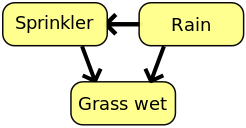
\includegraphics[width=0.4\textwidth]{bayes-net.png}
	\caption{By AnAj - http://en.wikipedia.org/wiki/File:SimpleBayesNet.svg, Public Domain, https://commons.wikimedia.org/w/index.php?curid=24448318}
	\label{im:Bayesnet}
\end{figure}

If we now observe e.g. $P(G)$ (which is $P(G|S,R)$) then we can apply Bayes' theorem to calculate $P(S|R)$ and $P(R)$.

\subsubsection{Curve fitting using Bayesian Networks}
While Bayesian Networks cannot be used to fit a curve directly, they can make calculating the probability of the parameters (likelihood) given the observed data easier.
In order to build the network for this use case we simply recall that all data points are random variables depending on $\mathbf{w}$, which is our set of parameters.
This is shown in \Cref{im:dependency}

\begin{figure}[h]
	\center
	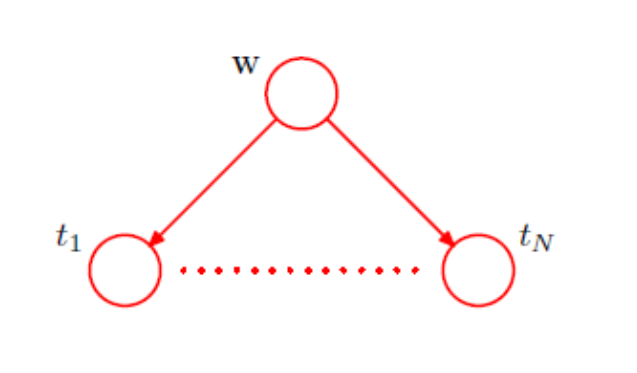
\includegraphics[width=0.4\textwidth]{dependency.png}
	\caption{Dependency of the data points on the parameters}
	\label{im:dependency}
\end{figure}

In Bayesian Networks repeating variables are often combined using a blue box like the one visible in \Cref{im:parameters} to save space.
\Cref{im:parameters} also contains the variables the parameters themselves depend on, as well as the standard deviation $\sigma^2$.

\begin{figure}[h]
	\center
	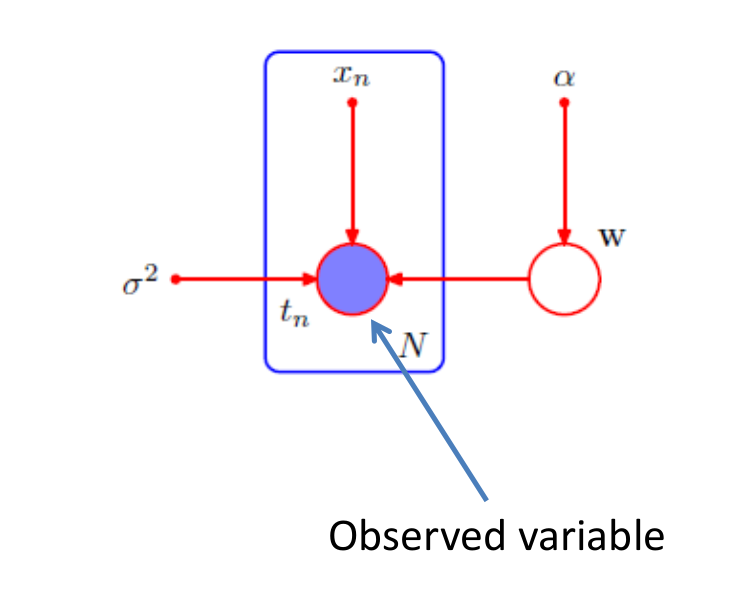
\includegraphics[width=0.6\textwidth]{bnet-parameters.png}
	\caption{Calculating the likelihood of a given parameter set using a Bayesian network}
	\label{im:parameters}
\end{figure}

\subsubsection{Conditional Independence}
Conditional Independence can be read directly from the structure of a Bayesian Network, using a process called D-separation.
For D-separation we utilize the fact that there are three possible ways two nodes can be directly related: Head-to-Head, Head-to-Tail and Tail-to-Tail.
The possibilities are shown in figure \Cref{im:relations}.

\begin{figure}[h]
	\centering
	\begin{subfigure}[b]{0.3\textwidth}
		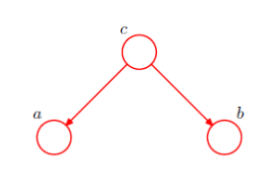
\includegraphics[width=\textwidth]{hth.png}
		\caption{Head-to-Head}
	\end{subfigure}
	\begin{subfigure}[b]{0.3\textwidth}
		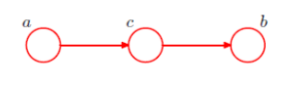
\includegraphics[width=\textwidth]{htt.png}
		\caption{Head-to-Tail}
	\end{subfigure}
	\begin{subfigure}[b]{0.3\textwidth}
		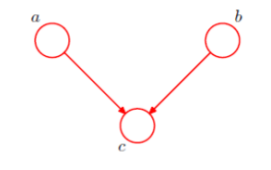
\includegraphics[width=\textwidth]{ttt.png}
		\caption{Tail-to-Tail}
	\end{subfigure}
	\caption{The possible relations in Bayesian networks}
	\label{im:relations}
\end{figure}

Now, for actually determining whether or not two variables are conditionally independent we consider the path between them in the Bayesian Network.
They are independent iff the path is blocked, and vice versa.

Let's consider the case of a Head-to-Head connection.
If $c$ is unobserved, the path is unblocked, which can be proven by marginalizing over $c$:
\begin{equation}
	p(a,b) = \sum_c p(a|c) p(b|c) p(c) \neq \sum_c p(a|c) p(b|c) \quad \rightarrow \quad a \nbigCI b\ |\ \emptyset
\end{equation}
As soon as $c$ is observed however, this path becomes blocked:
\begin{equation}
	p(a,b|c) = \frac{p(a,b,c)}{p(c)} = \frac{p(a|c) p(b|c) p(c)}{p(c)} = p(a|c) p(b|c) \quad \rightarrow \quad a \bigCI b\ |\ c
\end{equation}

The case for Head-to-Tail relationships is very similar, and also becomes blocked as $c$ is observed.
Tail-to-Tail relationships are different, as they become \emph{unblocked} as $c$ is observed.

\subsubsection{Markov Blanket or Markov Boundary}
The Markov Blanket for node $x_n$ is the set of all nodes (parents and children) that $x_n$ depends on.
This means that fixing all nodes in the Markov Blanket of $x_n$ allows us to calculate $x_n$, and splits it from the rest of the graph.
By doing this repeatedly (especially in the case of directed relationships), we can fix all values by starting from our observations.
The possibility of easily seeing where this is applicable is what makes graphical models so powerful.

\subsection{Markov Random Fields}

\subsection{Mixture of Gaussians}

\subsection{Restricted Boltzmann Machines}

\subsection{Neural Networks}

\end{document}
